\section{Casi d'uso}

	\subsection{Introduzione}
Il numero limitato dei casi d'uso\glo identificati è dovuto alla natura del prodotto, in quanto si tratta di un plugin e quindi di un'estensione di una piattaforma già esistente che viene integrata da un tool di addestramento esterno.
Per la piattaforma in questione non è fornita alcuna documentazione in quanto essa è già disponibile al sito web del distributore della piattaforma: \emph{Grafana Labs} (\href{https://grafana.com/docs/grafana/latest/}{Grafana Documentation}).

	\subsection{Struttura}
Viene riportata di seguito la classificazione dei casi d'uso. Verranno descritti nel documento rispettando la struttura esposta di seguito.
		\begin{itemize}
			\item diagramma UML (se presente);
			\item codice identificativo;
			\item titolo;
			\item attore primario;
			\item descrizione;
			\item precondizioni;
			\item postcondizioni;
			\item scenario principale;
			\item estensioni (se presenti);
			\item inclusioni (se presenti).
		\end{itemize}
Verrà utilizzato il linguaggio di modellazione UML 2.0\glo.
Ogni requisito può essere inserito in vari UC\glo, che si differenziano ciascuno per una diversa profondità dei dettagli da cui possono distinguersi ulteriori requisiti.

\subsection{Classificazione}
Identificare i casi d'uso in modo univoco aiuta la tracciabilità. I casi d'uso sono classificati nel seguente modo: \\
\centerline{\textbf{UC[codice\_padre].[codice\_figlio]}} \\
Il \textit{codice\_padre} è il codice univoco che rappresenta il requisito del caso d'uso. Se lo UC è collegato per profondità di dettaglio ad un altro UC, il \textit{codice\_figlio} verrà rappresentato in maniera gerarchica (esempio: se uno UC rappresenta un livello di dettaglio maggiore con \textit{codice\_padre} x, il suo codice sarà x.y, dove y indica l'annidamento raggiunto). \\ Verranno presentati prima i casi d'uso principali (da \hyperref[par:UC1]{UC1} a \hyperref[par:UC10]{UC10}), seguiti da quelli relativi ad estensioni (da \hyperref[par:UC11]{UC11} a \hyperref[par:UC18]{UC18}).

	\subsection{Attori}
Il sistema di autenticazione e registrazione dell'utente viene gestito per intero dal sistema Grafana, in quanto il prodotto finale non disporrà di una funzionalità di autenticazione/registrazione interna.									
Il numero limitato di differenti attori che si approcciano a parte del prodotto in analisi è dovuto principalmente al fatto che, essendo il prodotto \emph{Predire in Grafana} costituito da un plugin del sistema indipendente di Grafana ed un tool di addestramento, un esiguo numero di utenti hanno effettivamente la possibilità di approcciarsi al monitoraggio dei dati.
Per poter usare al meglio il tool di addestramento è consigliabile che l'utente disponga di nozioni di Machine Learning. Per sfruttare al meglio il plugin si raccomanda conoscenza riguardo il monitoraggio dei dati e di saper interpretare le previsioni visualizzate sulla dashboard. 
Inoltre non è necessaria la  registrazione degli utenti poiché l'addestramento avviene in un tool esterno.


	\subsubsection{Attori primari}
Essendo il prodotto finale un plugin open-source\glo è accessibile ad ogni tipo di utente. L'attore primario individuato è l'utente generico.
	\subsubsection{Attori secondari}
	\begin{itemize}
		\item\textbf{Piattaforma Grafana}: è un sistema di monitoraggio di stream\glo di dati, che ospiterà il plugin prodotto. Consente agli utenti registrati di lanciare alert e realizzare grafici modellati sui dati forniti in ingresso al plugin.
	\end{itemize}

% - Casi d'uso: Principali - %%%%%%%%%%%%%%%%%%%%%%%%%%%%%%%%%%%

	\label{par:UC1}
	\subsection{UC1 - Creazione file JSON dai dati di addestramento}

	\begin{figure}[H]
		\centering
		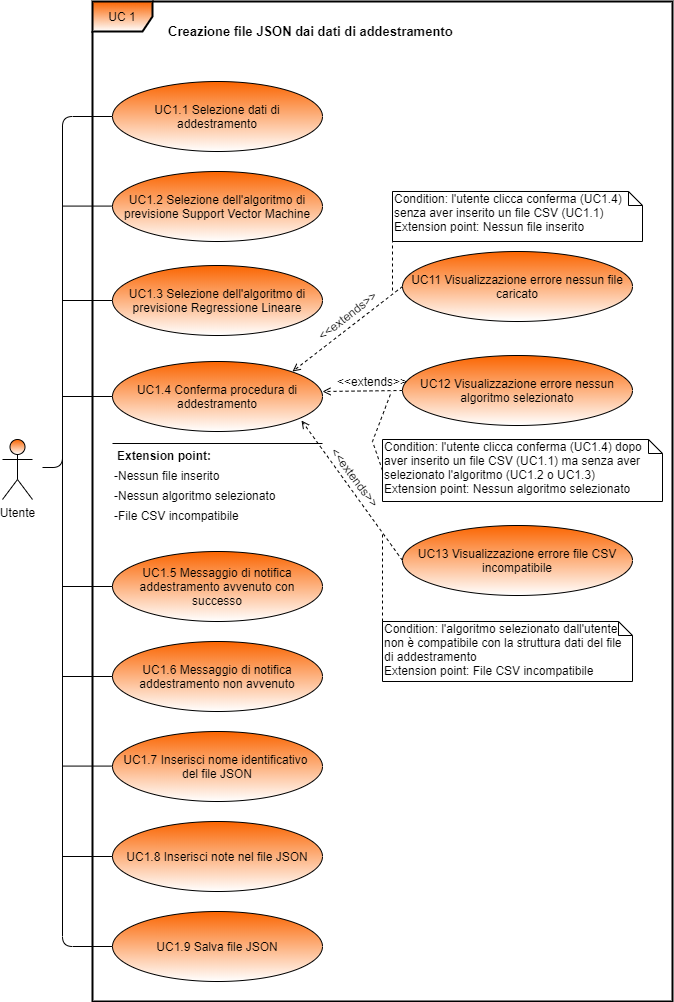
\includegraphics[scale=0.70]{../Analisi_dei_requisiti/img/Diagrammi_UML/UC1_tool_di_addestramento.png}
		\caption{Creazione file JSON dai dati di addestramento}
	\end{figure}	


		\begin{itemize}
			\item\textbf{Codice Identificativo}: UC1;
			\item\textbf{Titolo}: Creazione file JSON dai dati di addestramento;
			\item\textbf{Attore primario}: utente generico;
			\item\textbf{Descrizione}: attività di addestramento di un algoritmo di previsione presente in un applicativo esterno alla piattaforma Grafana\glo utilizzabile da qualsiasi utente che disponga di un file CSV contenente dei dati da utilizzare per l'addestramento;
			\item\textbf{Precondizioni}: l'utente si trova sull'applicativo esterno contenente il tool di addestramento;
			\item\textbf{Postcondizioni}:
				\begin{enumerate}
					\item viene addestrato l'algoritmo in base al CSV inserito;
					\item l'utente ha prodotto il file JSON contenente i predittori dell'algoritmo addestrato utilizzabile nel plugin \textit{"Predire in Grafana"}.
				\end{enumerate}
			\item\textbf{Scenario principale}:
				\begin{enumerate}
					\item (\hyperref[par:UC1.1]{UC1.1}) l'utente seleziona i dati di addestramento da caricare;
					\item (\hyperref[par:UC1.2]{UC1.2}) l'utente seleziona l'algoritmo di previsione "Support Vector Machine" dalla Combo Box\glo;
					\item (\hyperref[par:UC1.3]{UC1.3}) l'utente seleziona l'algoritmo di previsione "Regressione Lineare" dalla Combo Box\glo;
					\item (\hyperref[par:UC1.4]{UC1.4}) conferma delle operazioni;
					\item (\hyperref[par:UC1.5]{UC1.5}) viene visualizzato a schermo un messaggio di notifica di avvenuto successo della procedura di addestramento se tutto è stato eseguito correttamente;
					\item (\hyperref[par:UC1.6]{UC1.6}) viene visualizzato a schermo un messaggio di alert addestramento non riuscito se si sono verificati imprevisti durante la procedura di addestramento;
					\item (\hyperref[par:UC1.7]{UC1.7}) l'utente scarica l'addestramento ricevendo in output il file JSON contenente i predittori per SVM/RL che viene salvato localmente.
				\end{enumerate}
			\item\textbf{Estensioni}: 
				\begin{enumerate}
					\item \hyperref[par:UC11]{UC11} estende \hyperref[par:UC1.4]{UC1.4}: viene visualizzato un messaggio d'errore se non è stato caricato alcun file CSV contenente i dati di addestramento;
					\item \hyperref[par:UC12]{UC12} estende \hyperref[par:UC1.4]{UC1.4}: viene visualizzato un messaggio d'errore se non è stato scelto alcun algoritmo per l'addestramento;
					\item \hyperref[par:UC13]{UC13} estende \hyperref[par:UC1.4]{UC1.4}: viene visualizzato un messaggio d'errore se il file di addestramento è incompatibile con l'algoritmo scelto.
				\end{enumerate}
			
		\end{itemize}
		
		\label{par:UC1.1}
		\subsubsection{UC1.1 - Selezione dati di addestramento }
		\begin{itemize}
			\item\textbf{Codice Identificativo}: UC1.1;
			\item\textbf{Titolo}: Selezione dati di addestramento;
			\item\textbf{Attore primario}: utente generico;
			\item\textbf{Descrizione}: attività in cui viene inserito un file CSV contenente i dati utilizzati per l'addestramento;
			\item\textbf{Precondizioni}:
				\begin{enumerate}
					\item l'utente si trova sulla pagina web dedicata al tool di addestramento;
					\item l'utente deve possedere dei dati di addestramento\glo in un file formato CSV\glo;
					\item l'utente deve aver cliccato il pulsante di caricamento dati di addestramento.
				\end{enumerate}
			\item\textbf{Postcondizioni}: l'utente ha selezionato il file dei dati di addestramento;
			\item\textbf{Scenario principale}: l'utente seleziona il file CSV contenente i dati di addestramento dal file system ed è visibile solo il formato CSV.
		\end{itemize}
		
		\label{par:UC1.2}
		\subsubsection{UC1.2 - Selezione dell'algoritmo di previsione "Support Vector Machine"}
		\begin{itemize}
			\item\textbf{Codice Identificativo}: UC1.2;
			\item\textbf{Titolo}: Selezione dell'algoritmo di previsione "Support Vector Machine";
			\item\textbf{Attore primario}: utente generico;
			\item\textbf{Descrizione}: attività in cui viene scelto di addestrare una support vector machine come algoritmo di previsione;
			\item\textbf{Precondizioni}: l'utente deve aver selezionato i dati di addestramento (\hyperref[par:UC1.1]{UC1.1}) e si trova sulla Combo Box di selezione dell'algoritmo da addestrare;
			\item\textbf{Postcondizioni}: l'utente ha scelto di addestrare l'algoritmo "Support Vector Machine";
			\item\textbf{Scenario principale}: l'utente seleziona dalla Combo Box l'algoritmo di previsione "Support Vector Machine".
		\end{itemize}
		
		\label{par:UC1.3}
		\subsubsection{UC1.3 - Selezione dell'algoritmo di previsione "Regressione Lineare"}
		\begin{itemize}
			\item\textbf{Codice Identificativo}: UC1.2.1;
			\item\textbf{Titolo}: Selezione dell'algoritmo di previsione "Regressione Lineare";
			\item\textbf{Attore primario}: utente generico;
			\item\textbf{Descrizione}: attività in cui viene scelto di addestrare una regressione lineare come algoritmo di previsione;
			\item\textbf{Precondizioni}: l'utente deve aver selezionato i dati di addestramento (\hyperref[par:UC1.1]{UC1.1}) e si trova sulla Combo Box di selezione dell'algoritmo da addestrare;
			\item\textbf{Postcondizioni}: l'utente ha scelto di addestrare l'algoritmo "Regressione Lineare";
			\item\textbf{Scenario principale}: l'utente seleziona dalla Combo Box l'algoritmo di previsione "Regressione Lineare".		
		\end{itemize}
		
	\label{par:UC1.4}
	\subsubsection{UC1.4 - Conferma procedura addestramento}
		\begin{itemize}
			\item\textbf{Codice Identificativo}: UC1.4;
			\item\textbf{Titolo}: Conferma procedura addestramento;
			\item\textbf{Attore primario}: utente generico;
			\item\textbf{Descrizione}: attività in cui viene avviato l'addestramento dell'algoritmo scelto precedentemente in \hyperref[par:UC1.2]{UC1.2} utilizzando i dati caricati dopo aver completato \hyperref[par:UC1.1]{UC1.1};
			\item\textbf{Precondizioni}:
				\begin{enumerate}
					\item l'utente deve aver caricato i dati di addestramento (\hyperref[par:UC1.1]{UC1.1});
					\item l'utente deve aver selezionato l'algoritmo che vuole utilizzare per la previsione (\hyperref[par:UC1.2]{UC1.2}).
				\end{enumerate}
			\item\textbf{Postcondizioni}:
				\begin{enumerate}
					\item l'utente ha confermato la scelta dell'algoritmo e l'inserimento dei dati di addestramento;
					\item l'utente ha addestrato l'algoritmo e può scaricare il file JSON.
				\end{enumerate}
			\item\textbf{Scenario principale}: l'utente clicca il pulsante con etichetta "Avvia addestramento";
			\item\textbf{Estensioni}:
			\begin{enumerate}
				\item \hyperref[par:UC11]{UC11}: viene visualizzato un messaggio d'errore se non è stato caricato alcun file CSV contenente i dati di addestramento;
				\item \hyperref[par:UC12]{UC12}: viene visualizzato un messaggio d'errore se non è stato scelto alcun algoritmo per l'addestramento;
				\item \hyperref[par:UC13]{UC13}: viene visualizzato un messaggio d'errore se il file di addestramento è incompatibile con l'algoritmo scelto.
			\end{enumerate}
			 
						
		\end{itemize}
		
	\label{par:UC1.5}
	\subsubsection{UC1.5 - Visualizzazione messaggio di notifica "Addestramento avvenuto con successo"}
		\begin{itemize}
			\item\textbf{Codice Identificativo}: UC1.5;
			\item\textbf{Titolo}: Visualizzazione messaggio di notifica "Addestramento avvenuto con successo";
			\item\textbf{Attore primario}: utente generico;
			\item\textbf{Descrizione}: attività in cui viene visualizzato un messaggio in cui viene notificato che l'addestramento è avvenuto con successo;
			\item\textbf{Precondizioni}: 
				\begin{enumerate}
					\item l'utente ha inserito un file CSV compatibile (\hyperref[par:UC1.1]{UC1.1});
					\item l'utente ha selezionato un algoritmo compatibile con il CSV  (\hyperref[par:UC1.2]{UC1.2}).
				\end{enumerate}
			\item\textbf{Postcondizioni}: l'utente visualizza la notifica di addestramento avvenuto con successo;					
			\item\textbf{Scenario principale}:
				\begin{enumerate}
					\item l'utente visualizza il messaggio di notifica "Addestramento avvenuto con successo" in cui viene notificato che l'addestramento confermato(\hyperref[par:UC1.4]{UC1.4}) dell'algoritmo selezionato, a partire dai dati di addestramento, è avvenuto correttamente;
					\item l'utente clicca il pulsante "Conferma" per proseguire.		
				\end{enumerate}		
		\end{itemize}
		
	\label{par:UC1.6}
	\subsubsection{UC1.6 - Visualizzazione messaggio di alert "Addestramento non riuscito"}
		\begin{itemize}
			\item\textbf{Codice Identificativo}: UC1.6;
			\item\textbf{Titolo}: Visualizzazione messaggio di alert "Addestramento non riuscito";
			\item\textbf{Attore primario}: utente generico;
			\item\textbf{Descrizione}: attività in cui viene visualizzato un messaggio in cui viene segnalato che l'addestramento non è andato a buon fine a causa di un errore nella procedura di addestramento;
			\item\textbf{Precondizioni}: si è verificato un problema durante l'addestramento;
			\item\textbf{Postcondizioni}: l'utente visualizza il messaggio di alert di addestramento non riuscito;					
			\item\textbf{Scenario principale}:
				\begin{enumerate}
				\item l'utente visualizza il messaggio di alert "Addestramento non riuscito" in cui viene segnalato che non è stato possibile addestrare l'algoritmo perché è stato caricato un CSV incompatibile (\hyperref[par:UC12]{UC12}) oppure nel caso in cui non sia stato scelto l'algoritmo da addestrare (\hyperref[par:UC11]{UC11}) o caricato alcun file CSV (\hyperref[par:UC10]{UC10});
				\item l'utente clicca il pulsante "Conferma" per proseguire.
					
				\end{enumerate}
				
					
				
					
		\end{itemize}

	\label{par:UC1.7}
	\subsubsection{UC1.7 - Salvataggio file JSON}
		\begin{itemize}
			\item\textbf{Codice Identificativo}: UC1.7;
			\item\textbf{Titolo}: Salvataggio file JSON;
			\item\textbf{Attore primario}: utente generico;
			\item\textbf{Descrizione}: attività in cui viene scaricato nel proprio file-system il file JSON contenente l'algoritmo addestrato;
			\item\textbf{Precondizioni}: l'utente ha cliccato il pulsante di conferma (\hyperref[par:UC1.4]{UC1.4});
			\item\textbf{Postcondizioni}: l'utente ha salvato il file JSON in locale;
			\item\textbf{Scenario principale}: l'utente scarica il file JSON che è stato prodotto cliccando il pulsante di download; tale pulsante è visibile solo se la procedura di addestramento è stata confermata con successo. 	
			
			 	
		\end{itemize}

%%%%%%%%%%%%%%%%%%%%%%%%%%%%%%%

	\label{par:UC2}
	\subsection{UC2 - Caricamento del file JSON nel plugin}
	
	%\begin{figure}[H]
	%	\centering
	%	\includegraphics[scale=0.70]{../Analisi_dei_requisiti/img/Diagrammi_UML/UC2_Caricamento_file_JSON_nel_plugin.png}
	%	\caption{Caricamento del file JSON}
	%\end{figure}	
		
		\begin{itemize}
			\item\textbf{Codice Identificativo}: UC2;
			\item\textbf{Titolo}: Caricamento del file JSON nel plugin;
			\item\textbf{Attore primario}: utente generico;
			\item\textbf{Descrizione}: attività in cui viene caricato nel plugin \textit{Predire in Grafana} un file JSON contenente un algoritmo addestrato. Il plugin si occuperà di trattare l'algoritmo addestrato automaticamente, per effettuare previsioni in base all'algoritmo presente nel file JSON, motivo per cui non è necessario specificare ulteriormente se si tratti di una Support Vector Machine o Regressione Lineare. Non è possibile addestrare tale algoritmo direttamente nella piattaforma Grafana; 
			\item\textbf{Precondizioni}:
				\begin{enumerate}
					\item l'utente ha effettuato l'accesso alla piattaforma Grafana;
					\item l'utente ha selezionato una dashboard e ha aggiunto il plugin \textit{Predire in Grafana} come visualizzazione, le cui operazioni verranno riportate sul rispettivo pannello;
					\item l'utente dispone del file JSON contenente i predittori e la definizione dell'algoritmo addestrato (\hyperref[par:UC1]{UC1}). Tale JSON deve essere compatibile, altrimenti non viene caricato.
				\end{enumerate}
			\item\textbf{Postcondizioni}:
				\begin{enumerate}
					\item l'utente ha caricato il file JSON con predittori associati nel plugin;
					\item viene letta la definizione del predittore dal file in formato JSON.
				\end{enumerate}
			\item\textbf{Scenario principale}:
				\begin{enumerate}
					\item (\hyperref[par:UC2.1]{UC2.1}) l'utente seleziona il file JSON contenente i predittori da locale;
					\item (\hyperref[par:UC2.2]{UC2.2}) l'utente conferma il caricamento;
					\item (\hyperref[par:UC2.3]{UC2.3}) viene visualizzato a schermo un messaggio di notifica di avvenuto successo della procedura di caricamento JSON.
					\item (\hyperref[par:UC2.4]{UC2.4}) viene visualizzato il contenuto del file JSON appena caricato.
				\end{enumerate}
			%\item\textbf{Estensioni}:
			%	\begin{enumerate}
				%REMOVE%
					%\item\hyperref[par:UC13]{UC13} estende \hyperref[par:UC2.1]{UC2.1}: viene visualizzato un messaggio di alert nel caso in cui sia già presente un file JSON caricato nel plugin \textit{Predire in Grafana};
					%\item\hyperref[par:UC14]{UC14} estende \hyperref[par:UC2.2]{UC2.2}: viene visualizzato un messaggio d'errore nel caso in cui l'operazione di caricamento del file non sia andata a buon fine.
				%\end{enumerate}	
			
		\end{itemize}
		
		
		\label{par:UC2.1}
		\subsubsection{UC2.1 - Selezione del file JSON}
		\begin{itemize}
			\item\textbf{Codice Identificativo}: UC2.1;
			\item\textbf{Titolo}: Selezione del file JSON;
			\item\textbf{Attore primario}: utente generico;
			\item\textbf{Descrizione}: attività in cui viene selezionato il file JSON, contenente l'algoritmo addestrato, da locale che andrà ad essere importato nel plugin;
			\item\textbf{Precondizioni}:
				\begin{enumerate}
					\item l'utente visualizza il pannello \textit{Predire in Grafana} nella dashboard;
					\item l'utente ha cliccato il pannello di selezione del file.
					\end{enumerate}
			\item\textbf{Postcondizioni}: l'utente ha selezionato il file JSON;
			\item\textbf{Scenario principale}: l'utente seleziona dalla finestra di selezione il file JSON da importare tra quelli disponibili. Sono visibili solo i file con formato .json;
			%REMOVE%
			%\item\textbf{Estensioni}: \hyperref[par:UC13]{UC13}: viene visualizzato un messaggio di alert nel caso in cui sia già presente un file JSON caricato nel plugin \textit{Predire in Grafana}.		
			\end{itemize}
		
		\label{par:UC2.2} 
		\subsubsection{UC2.2 - Conferma di caricamento}
		\begin{itemize}
			\item\textbf{Codice Identificativo}: UC2.2;
			\item\textbf{Titolo}: Conferma di caricamento;
			\item\textbf{Attore primario}: utente generico;
			\item\textbf{Descrizione}: attività in cui viene confermata la selezione del file JSON da importare nel plugin;
			\item\textbf{Precondizioni}: l'utente ha selezionato il file JSON da caricare;
			\item\textbf{Postcondizioni}: l'utente ha caricato il file nel plugin;
			\item\textbf{Scenario principale}: l'utente clicca il pulsante etichettato con "Apri" e il file viene caricato;
			%\item\textbf{Estensioni}: \hyperref[par:UC13]{UC13}: viene visualizzato un messaggio d'errore nel caso in cui l'operazione di caricamento del file non sia andata a buon fine.
					
		\end{itemize}
		
		\label{par:UC2.3}
	\subsubsection{UC2.3 - Visualizzazione messaggio di notifica "Caricamento file JSON avvenuto successo"}
		\begin{itemize}
			\item\textbf{Codice Identificativo}: UC2.3;
			\item\textbf{Titolo}: Visualizzazione messaggio di notifica "Caricamento file JSON avvenuto con successo";
			\item\textbf{Attore primario}: utente generico;
			\item\textbf{Descrizione}: attività in cui viene visualizzato un messaggio in cui viene notificato che il file JSON è stato importato con successo;
			\item\textbf{Precondizioni}: l'utente ha confermato il caricamento del file JSON selezionato (\hyperref[par:UC2.2]{UC2.2});
			\item\textbf{Postcondizioni}: l'utente ha visualizzato la notifica di avvenuto caricamento del file JSON nel plugin;
			\item\textbf{Scenario principale}:
				\begin{enumerate}
					\item l'utente visualizza il messaggio di notifica "Caricamento file JSON avvenuto con successo" in cui viene notificato che il caricamento (\hyperref[par:UC2]{UC2}) è avvenuto correttamente;
					\item l'utente clicca il pulsante "X" per proseguire.		
				\end{enumerate}		
		\end{itemize}
		
		\label{par:UC2.4}
	\subsubsection{UC2.4 - Visualizzazione contenuto file JSON}
		\begin{itemize}
			\item\textbf{Codice Identificativo}: UC2.4;
			\item\textbf{Titolo}: Visualizzazione contenuto file JSON";
			\item\textbf{Attore primario}: utente generico;
			\item\textbf{Descrizione}: attività in cui viene visualizzato il contenuto del file JSON appena caricato nel plugin;
			\item\textbf{Precondizioni}: 
				\begin{enumerate}
					\item l'utente ha confermato il caricamento del file JSON selezionato (\hyperref[par:UC2.2]{UC2.2});
					\item l'utente ha visualizzato il messaggio di notifica "Caricamento file JSON avvenuto con successo" (\hyperref[par:UC2.3]{UC2.3}).
				\end{enumerate}
			\item\textbf{Postcondizioni}: l'utente ha visualizza il contenuto del file JSON caricato;
			\item\textbf{Scenario principale}: l'utente visualizza il contenuto del file JSON appena caricato dove può esaminare le informazioni relative a:
			\begin{itemize}
			\item autore del file;
			\item versione dell'applicativo di addestramento esterno;
			\item algoritmo addestrato;
			\item data di creazione del file;
			\item identificativi dei predittori;
			\item risultati dell'addestramento utilizzati nel calcoli di previsione;
			\item formula della retta di regressione.
\end{itemize}			
			
		\end{itemize}

%%%%%%%%%%%%%%%%%%%%%%%%%%%%%%%

	\label{par:UC3}
	\subsection{UC3 - Collegamento del predittore al flusso dati}

		%\begin{figure}[H]
		%\centering
		%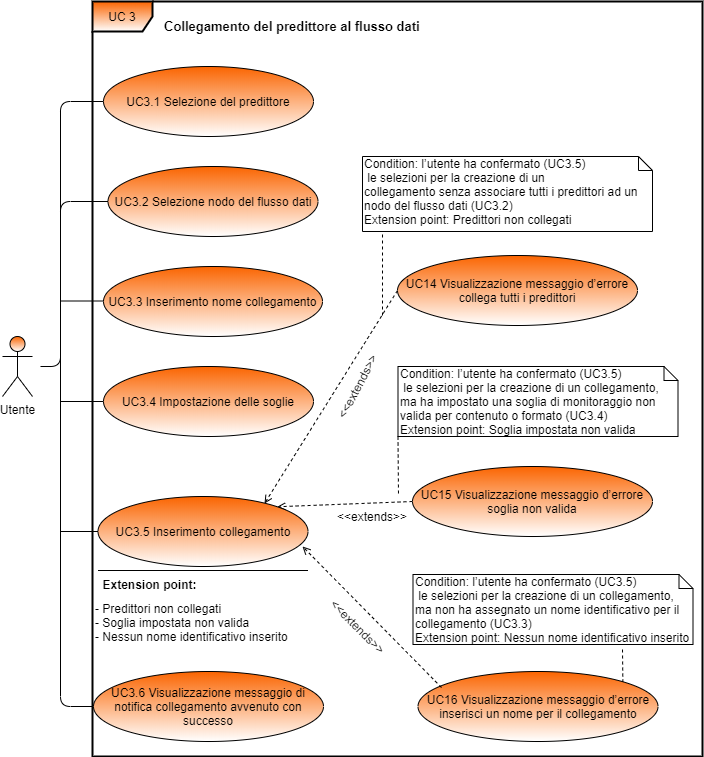
\includegraphics[scale=0.70]{../Analisi_dei_requisiti/img/Diagrammi_UML/UC3_collegamento_flusso_dati.png}
		%\caption{Collegamento del predittore al flusso dati}
		%\end{figure}	

		\begin{itemize}
			\item\textbf{Codice Identificativo}: UC3;
			\item\textbf{Titolo}: Collegamento del predittore al flusso dati;
			\item\textbf{Attore primario}: utente generico;
			\item\textbf{Descrizione}: attività in cui viene creato un collegamento tra predittore e nodo del flusso dati selezionati. Ogni collegamento creato dall'utente sarà disponibile per modifiche e cancellazioni in una lista di collegamenti;
			\item\textbf{Precondizioni}:
				\begin{enumerate}
					\item l'utente ha caricato e letto con successo i predittori contenuti nel file JSON (\hyperref[par:UC2]{UC2});
					\item l'utente dispone di una serie di predittori da poter collegare al flusso di dati voluto;
					\item l’utente deve aver configurato la connessione al server tramite Grafana;
					\item l’utente deve disporre di almeno un database caricato in Grafana contenente una tabella con i dati su cui fare le previsioni e deve aver registrato almeno una query sul database.
					

					
				\end{enumerate}
			\item\textbf{Postcondizioni}: l'utente ha collegato correttamente ciascun predittore ad un flusso dati creando un collegamento identificato da un nominativo assegnato sempre dall'utente, definendo dove desiderato le soglie per i rispettivi stati di ogni nodo e visualizza i collegamenti in un pannello dedicato;
			\item\textbf{Scenario principale}:
				\begin{enumerate}
					\item (\hyperref[par:UC3.1]{UC3.1}) l'utente seleziona il predittore a cui collegare un nodo del flusso. I predittori sono disponibili una volta caricato il file JSON;
					\item (\hyperref[par:UC3.2]{UC3.2}) l'utente seleziona il nodo del flusso dati da associare al predittore attraverso una query\glo;
					\item (\hyperref[par:UC3.3]{UC3.3}) l'utente inserisce un nome identificativo per il collegamento che andrà ad inserire;
					\item (\hyperref[par:UC3.4]{UC3.4}) impostazione delle soglie dove desiderato;
					\item (\hyperref[par:UC3.5]{UC3.5}) l'utente conferma le impostazioni di collegamento selezionate provando a inserire il collegamento nella lista dei collegamenti;	
					\item (\hyperref[par:UC3.6]{UC3.6}) viene visualizzata una notifica avvenuto collegamento al nodo del flusso dati se la procedura è andata a buon fine;
				\end{enumerate}
			\item\textbf{Estensioni}:
				\begin{enumerate}
				\item\hyperref[par:UC14]{UC14} estende \hyperref[par:UC3.5]{UC3.5}: viene visualizzato un messaggio d'errore nel caso non siano stati associati tutti i predittori ad un nodo del flusso dati;
					\item\hyperref[par:UC15]{UC15} estende \hyperref[par:UC3.5]{UC3.5}: viene visualizzato un messaggio di errore soglia non valida nel caso venga inserito un valore non consentito;
					\item\hyperref[par:UC16]{UC16} estende \hyperref[par:UC3.5]{UC3.5}: viene visualizzato un messaggio d'errore nel caso non sia stato inserito un nome identificativo per il collegamento;
					
						
				\end{enumerate}
		\end{itemize}
		

		\label{par:UC3.1}
		\subsubsection{UC3.1 - Selezione del predittore}
		\begin{itemize}
			\item\textbf{Codice Identificativo}: UC3.1;
			\item\textbf{Titolo}: Selezione del predittore;
			\item\textbf{Attore primario}: utente generico;
			\item\textbf{Descrizione}: attività in cui viene selezionato il predittore da associare ad un nodo del flusso dati;
			\item\textbf{Precondizioni}: è stato letto il file JSON con i predittori e l'utente visualizza una lista con i predittori disponibili;
			\item\textbf{Postcondizioni}: è stato scelto il predittore tra quelli disponibili presenti sulla lista;
			\item\textbf{Scenario principale}: l'utente seleziona il predittore che intende associare ad un aspetto del flusso.
		\end{itemize}
		
	
	\label{par:UC3.2}
	\subsubsection{UC3.2 - Selezione nodo del flusso dati}
		\begin{itemize}
			\item\textbf{Codice Identificativo}: UC3.2;
			\item\textbf{Titolo}: Selezione nodo del flusso dati;
			\item\textbf{Attore primario}: utente generico;
			\item\textbf{Descrizione}: attività in cui viene selezionato il nodo del flusso dati che viene associato al predittore selezionato;
			\item\textbf{Precondizioni}:
				\begin{enumerate}
					\item il predittore da collegare è stato selezionato dalla lista dei predittori (\hyperref[par:UC3.1]{UC3.1});
					\item sono state aggiunte delle query al sistema di Grafana;
					\item l'utente visualizza la lista di nodi del flusso di dati a cui poter associare il predittore selezionato.
				\end{enumerate}
			\item\textbf{Postcondizioni}: per ogni predittore della lista l'utente ha selezionato il nodo dal flusso dati da associare;
		
			\item\textbf{Scenario principale}: l'utente seleziona l'aspetto interessato dal flusso di dati al quale può essere agganciato il predittore selezionato in precedenza.
		\end{itemize}
		
	\subsubsection{UC3.3 - Inserimento nome identificativo per il collegamento}
		\begin{itemize}
			\item\textbf{Codice Identificativo}: UC3.3;
			\item\textbf{Titolo}: Inserimento nome identificativo per il collegamento;
			\item\textbf{Attore primario}: utente generico;
			\item\textbf{Descrizione}: attività in cui viene assegnato un nome identificativo al collegamento che verrà creato;
			\item\textbf{Precondizioni}:
				\begin{enumerate}
					\item il predittore da collegare è stato selezionato dalla lista dei predittori (\hyperref[par:UC3.1]{UC3.1});
					\item il nodo del flusso dati da collegare è stato selezionato dalla lista delle query disponibili (\hyperref[par:UC3.2]{UC3.2});
					
				\end{enumerate}
			\item\textbf{Postcondizioni}: l'utente ha assegnato un nome identificativo per il collegamento che verrà creato alla conferma delle operazioni di collegamento;
		
			\item\textbf{Scenario principale}: l'utente inserisce un nominativo nel form con etichetta "Nome del collegamento" che andrà ad identificare il collegamento;
		\end{itemize}
			

	\label{par:UC3.4}
	\subsubsection{UC3.4 - Impostazione delle soglie}
		\begin{itemize}
			\item\textbf{Codice Identificativo}: UC3.4;
			\item\textbf{Titolo}: Impostazione delle soglie;
			\item\textbf{Attore primario}: utente generico;
			\item\textbf{Descrizione}: attività in cui viene impostata una soglia per il collegamento. Al superamento di tale soglia, durante la visualizzazione delle previsioni , verranno lanciati degli alert sulla dashboard;
			\item\textbf{Precondizioni}: l'utente ha associato i predittori della lista ad un flusso dati (\hyperref[par:UC3.1]{UC3.1});
			\item\textbf{Postcondizioni}: l'utente ha impostato la soglia di monitoraggio sui predittori;
			\item\textbf{Scenario principale}: l'utente aggiunge una soglia da associare. \'E possibile impostare una soglia minima e/o una soglia massima;
		\end{itemize}

	\label{par:UC3.5}
	\subsubsection{UC3.5 - Inserimento collegamento}
		\begin{itemize}
			\item\textbf{Codice Identificativo}: UC3.5;
			\item\textbf{Titolo}: Inserimento collegamento;
			\item\textbf{Attore primario}: utente generico;
			\item\textbf{Descrizione}: attività in cui vengono confermate le configurazioni per la creazione del collegamento che viene inserito in una lista di collegamenti disponibili per le previsioni;
			\item\textbf{Precondizioni}: l'utente ha creato le basi per l'associazione del predittore al nodo del flusso dati scelto. In particolare è stato selezionato il predittore (\hyperref[par:UC3.1]{UC3.1}), il nodo del flusso dati da associare (\hyperref[par:UC3.2]{UC3.2}), è stato assegnato un nome identificativo al collegamento(\hyperref[par:UC3.3]{UC3.3}) ed è stata impostata una eventuale soglia (\hyperref[par:UC3.4]{UC3.4});
			\item\textbf{Postcondizioni}:
				\begin{enumerate}
					\item l'utente ha inserito il nuovo collegamento e visualizza la lista dei collegamenti disponibili per le previsioni;
					\item l'utente ha la possibilità di effettuare un altro collegamento tornando a \hyperref[par:UC3.1]{UC3.1}.
				\end{enumerate}
			\item\textbf{Scenario principale}: l'utente clicca il pulsante etichettato con "Inserimento collegamento";
			\item\textbf{Estensioni}: 
				\begin{enumerate}
					\item\hyperref[par:UC14]{UC14}: viene visualizzato un messaggio d'errore nel caso non siano stati associati tutti i predittori ad un nodo del flusso dati;
					\item\hyperref[par:UC15]{UC15}: viene visualizzato un messaggio di errore "Soglia non valida" nel caso venga inserito un valore non consentito;			
					\item\hyperref[par:UC16]{UC16}: viene visualizzato un messaggio d'errore nel caso non sia stato inserito un nome identificativo per il collegamento.
					
				\end{enumerate}							
				
				
				
		\end{itemize}
		
	\label{par:UC3.6}
	\subsubsection{UC3.6 - Visualizzazione messaggio di notifica "Collegamento avvenuto con successo"}
		\begin{itemize}
			\item\textbf{Codice Identificativo}: UC3.6;
			\item\textbf{Titolo}: Visualizzazione messaggio di notifica "Collegamento avvenuto con successo";
			\item\textbf{Attore primario}: utente generico;
			\item\textbf{Descrizione}: attività in cui viene visualizzato un messaggio di successo della procedura di collegamento che determina la creazione del collegamento;
			\item\textbf{Precondizioni}: l'utente ha confermato il collegamento (\hyperref[par:UC3.5]{UC3.5});
			\item\textbf{Postcondizioni}: l'utente visualizza la notifica di avvenuto successo del collegamento;
			\item\textbf{Scenario principale}:
				\begin{enumerate}
					\item l'utente visualizza il messaggio di notifica "Collegamento avvenuto con successo" in cui viene notificato che il collegamento tra predittore e flusso dati (\hyperref[par:UC3]{UC3}) è avvenuto correttamente;
					\item l'utente clicca il pulsante "X" per proseguire.		
				\end{enumerate}		
		\end{itemize}
		
%%%%%%%%%%%%%%%%%%%%%%%%%%%%%%%

	\label{par:UC4}
	\subsection{UC4 - Visualizzazione pannello lista collegamenti}
		\begin{itemize}
			\item\textbf{Codice Identificativo}: UC4;
			\item\textbf{Titolo}: Visualizzazione pannello lista collegamenti;
			\item\textbf{Attore primario}: utente generico;
			\item\textbf{Descrizione}: attività in cui viene visualizzata la lista di tutti i collegamenti creati dall'utente fin a quel momento;
			\item\textbf{Precondizioni}: 
			\begin{enumerate}
			 	\item l'utente ha effettuato l'accesso alla piattaforma Grafana;
				\item l'utente ha selezionato una dashboard e ha aggiunto il plugin \textit{Predire in Grafana} come visualizzazione, le cui operazioni verranno riportate sul rispettivo pannello;
				\item per la visualizzazione dei collegamenti creati si suppone che l'utente abbia inserito almeno un collegamento correttamente (\hyperref[par:UC3]{UC3});
\end{enumerate}			
			\item\textbf{Postcondizioni}: l'utente visualizza un pannello contenente la lista di tutti i collegamenti effettuati. Se non sono presenti collegamenti la lista presenta un'etichetta "Nessun collegamento inserito". Ogni nuovo collegamento confermato viene aggiunto alla lista;
			\item\textbf{Scenario principale}: l'utente visualizza la lista di collegamenti effettuati correttamente fino a quel momento con le rispettive impostazioni di collegamento selezionate. Per ogni collegamento sono presenti i pulsanti "Modifica" e "Scollega" relativi alle operazioni di modifica delle impostazioni e eliminazione per il collegamento. Ogni collegamento è così suddiviso:
					\begin{itemize}
						\item nome identificativo del collegamento;
						\item nominativo del predittore selezionato (per tutti i predittori presenti);
						\item nominativo del nodo del flusso dati associato al predittore (per tutti i predittori presenti);
						\item impostazioni delle soglie inserite.
					\end{itemize}
							
		\end{itemize}

%%%%%%%%%%%%%%%%%%%%%%%%%%%%%%%%

\label{par:UC5}
	\subsection{UC5 - Scollegamento predittore}
	
	
	%\begin{figure}[H]
		%\centering
		%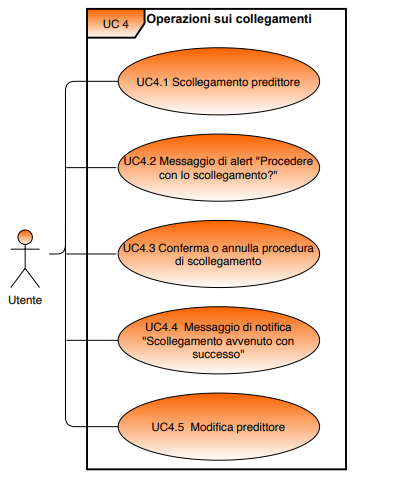
\includegraphics[scale=0.80]{../Analisi_dei_requisiti/img/Diagrammi_UML/UC4_Operazioni_sui_collegamenti.png}
		%\caption{Operazioni sui collegamenti} 
		%\end{figure}	

		\begin{itemize}
			\item\textbf{Codice Identificativo}: UC5;
			\item\textbf{Titolo}: Scollegamento predittore;
			\item\textbf{Attore primario}: utente generico;
			\item\textbf{Descrizione}: attività in cui viene eliminato un collegamento dalla lista dei collegamenti effettuati in precedenza;
			\item\textbf{Precondizioni}:
			\begin{enumerate}
			\item l'utente si trova sul pannello dedicato alla lista dei collegamenti tra predittore e
flusso dati (\hyperref[par:UC4]{UC4});
			\item  l'utente visualizza la lista dei collegamenti in cui è presente almeno un collegamento tra predittore e flusso dati.	
\end{enumerate}			
			\item\textbf{Postcondizioni}: 
			\begin{enumerate}
				\item l'utente ha scollegato il predittore dal nodo del flusso dati precedentemente associato;
				\item nella lista dei collegamenti non viene più visualizzato il collegament
				o che è stato
scollegato e quindi eliminato.
			\end{enumerate}
			l'utente ha rimosso il collegamento desiderato dalla lista dei collegamenti o ne ha annullato la rimozione;
			\item\textbf{Scenario principale}:
			\begin{enumerate}
				\item (\hyperref[par:UC5.1]{UC5.1}) l'utente clicca il pulsante con etichetta "Scollega";
				\item (\hyperref[par:UC5.2]{UC5.2}) l'utente visualizza un messaggio di alert "Scollegare il predittore?";
				\item (\hyperref[par:UC5.3]{UC5.3}) l'utente conferma lo scollegamento;
				\item (\hyperref[par:UC5.4]{UC5.4}) l'utente visualizza il messaggio di notifica di scollegamento avvenuto con successo;
				\item (\hyperref[par:UC5.5]{UC5.5}) l'utente annulla lo scollegamento;
			\end{enumerate}	
			\item\textbf{Estensioni}: \hyperref[par:UC17]{UC17} estende \hyperref[par:UC5.1]{UC5.1}: viene visualizzato un messaggio di errore sull'impossibilità di eliminazione del collegamento dovuta alla presenza di un monitoraggio sulle previsioni avviato.		
			\end{itemize}
			
			\label{par:UC5.1}
	\subsubsection{UC5.1 - Richiesta di scollegamento}
		\begin{itemize}
			\item\textbf{Codice Identificativo}: UC5.1;
			\item\textbf{Titolo}: Richiesta di scollegamento;
			\item\textbf{Attore primario}: utente generico;
			\item\textbf{Descrizione}: attività in cui viene cliccato il pulsante di scollegamento necessario per inviare la richiesta di eliminazione di un collegamento;
			\item\textbf{Precondizioni}: l'utente ha scelto dalla lista dei collegamenti visualizzata (\hyperref[par:UC4]{UC4}) il collegamento che vuole eliminare;
			\item\textbf{Postcondizioni}: l'utente ha cliccato il pulsante con etichetta "Scollega" utilizzato per eliminare un collegamento;
			\item\textbf{Scenario principale}: l'utente clicca il pulsante con etichetta "Scollega" utilizzato per eliminare il collegamento desiderato;
			\item\textbf{Estensioni}: \hyperref[par:UC17]{UC17}: viene visualizzato un messaggio di errore sull'impossibilità di eliminazione del collegamento dovuta alla presenza di un monitoraggio sulle previsioni avviato.					
	
		\end{itemize}		
		
		
	\label{par:UC5.2}
	\subsubsection{UC5.2 - Visualizzazione messaggio di alert "Scollegare predittore?"}
		\begin{itemize}
			\item\textbf{Codice Identificativo}: UC5.2;
			\item\textbf{Titolo}: Visualizzazione messaggio di alert "Scollegare predittore?";
			\item\textbf{Descrizione}: attività in cui l'utente visualizza un messaggio che lo interroga sul proseguimento dell'eliminazione di un collegamento;
			\item\textbf{Attore primario}: utente generico;
			\item\textbf{Precondizioni}: l'utente ha cliccato il pulsante di scollegamento "Scollega" (\hyperref[par:UC5.1]{UC5.1}) per il collegamento che ha intenzione di eliminare;
			\item\textbf{Postcondizioni}: l'utente ha visualizzato il messaggio di alert sul tentativo di scollegamento del predittore;
					
			\item\textbf{Scenario principale}: l'utente visualizza un messaggio di alert "Scollegare predittore?" in cui viene segnalato che è stata selezionata una procedura di scollegamento del predittore.
	
		\end{itemize}		
		
	\label{par:UC5.3}
	\subsubsection{UC5.3 - Conferma scollegamento}
		\begin{itemize}
			\item\textbf{Codice Identificativo}: UC5.3;
			\item\textbf{Titolo}: Conferma scollegamento;
			\item\textbf{Attore primario}: utente generico;
			\item\textbf{Descrizione}: attività in cui viene confermata dall'utente la richiesta di scollegamento del predittore intrapresa dallo stesso precedentemente;
			\item\textbf{Precondizioni}: l'utente ha visualizzato il messaggio di alert sul tentativo di scollegamento predittore;
			\item\textbf{Postcondizioni}: l'utente ha confermato la procedura di scollegamento;	
			\item\textbf{Scenario principale}: l'utente clicca il pulsante "Ok" per proseguire e scollegare il predittore procedendo in questo modo ad eliminare il collegamento desiderato.
			\end{itemize}
			
	\label{par:UC5.4}
	\subsubsection{UC5.4 - Visualizzazione messaggio di notifica "Scollegamento avvenuto con successo"}
		\begin{itemize}
			\item\textbf{Codice Identificativo}: UC5.4;
			\item\textbf{Titolo}: Visualizzazione messaggio di notifica "Scollegamento avvenuto con successo";
			\item\textbf{Attore primario}: utente generico;
			\item\textbf{Descrizione}: attività in cui viene visualizzato un messaggio di notifica che informa l'utente sulla riuscita dello scollegamento; 
			\item\textbf{Precondizioni}: 
				\begin{enumerate}
					\item l'utente ha confermato lo scollegamento del predittore (\hyperref[par:UC5.3]{UC5.3})
				\end{enumerate}
			\item\textbf{Postcondizioni}: l'utente ha visualizzato la notifica di scollegamento avvenuto con successo;				
			\item\textbf{Scenario principale}:
				\begin{enumerate}
					\item l'utente visualizza il messaggio di notifica "Scollegamento avvenuto successo" in cui viene notificato che lo scollegamento del predittore confermato(\hyperref[par:UC5.3]{UC5.3}) è avvenuto correttamente;
					\item l'utente clicca il pulsante "X" per proseguire.		
				\end{enumerate}		
		\end{itemize}

\label{par:UC5.5}
	\subsubsection{UC5.5 - Annullamento scollegamento}
		\begin{itemize}
			\item\textbf{Codice Identificativo}: UC5.5;
			\item\textbf{Titolo}: Conferma scollegamento;
			\item\textbf{Attore primario}: utente generico;
			\item\textbf{Descrizione}: attività in cui viene annullata dall'utente la richiesta di scollegamento del predittore intrapresa dallo stesso precedentemente;
			\item\textbf{Precondizioni}: l'utente ha visualizzato il messaggio di alert sul tentativo di scollegamento predittore;
			\item\textbf{Postcondizioni}: l'utente ha annullato la procedura di scollegamento;	
			\item\textbf{Scenario principale}: l'utente clicca il pulsante "Annulla" e viene riportato alla visualizzazione dei collegamenti (\hyperref[par:UC4]{UC4}).
			\end{itemize}
			
%%%%%%%%%%%%%%%%%%%%%%%%%%%%%%%%%%%%		
		
	\label{par:UC6}
	\subsection{UC6 - Modifica collegamento}
	
%	\begin{figure}[H]
%		\centering
%		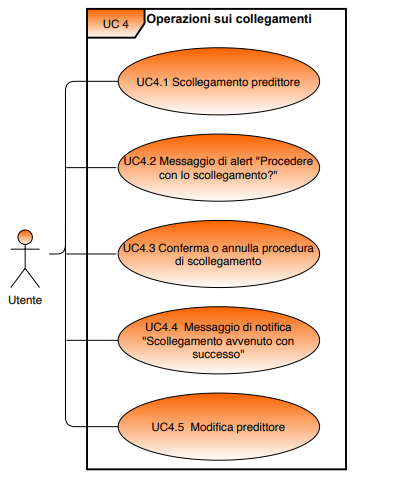
\includegraphics[scale=0.80]{../Analisi_dei_requisiti/img/Diagrammi_UML/UC4_Operazioni_sui_collegamenti.png}
%		\caption{Operazioni sui collegamenti} 
%		\end{figure}	


		\begin{itemize}
			\item\textbf{Codice Identificativo}: UC6;
			\item\textbf{Titolo}: Modifica collegamento;
			\item\textbf{Attore primario}: utente generico;
			\item\textbf{Descrizione}: attività in cui vengono modificate le impostazioni di un collegamento esistente. \'E possibile modificarne il nome identificativo o le associazioni tra predittore e nodo del flusso dati. Non è possibile modificare il collegamento se è stato avviato il monitoraggio delle previsioni;
			\item\textbf{Precondizioni}:
			\begin{enumerate}
			\item l'utente si trova sul pannello dedicato alla lista dei collegamenti tra predittore e
flusso dati (\hyperref[par:UC4]{UC4});
			\item  l'utente visualizza la lista dei collegamenti in cui è presente almeno un collegamento tra predittore e flusso dati;	
			\item il monitoraggio non deve esser stato avviato; nel caso sia stato avviato deve esser interrotto per poter procedere ().
			\end{enumerate}
							
			\item\textbf{Postcondizioni}:
			\begin{enumerate}
				\item l'utente ha modificato o annullato la modifica per le impostazioni del collegamento desiderato;
				\item nella lista dei collegamenti viene visualizzato il collegamento con le relative modifiche appena applicate.			
			
			\end{enumerate}
				
			\item\textbf{Scenario principale}:
				\begin{enumerate}
				
				\item (\hyperref[par:UC6.1]{UC6.1}) l'utente clicca il pulsante con etichetta "Modifica" e viene aperto un pannello con le informazioni modificabili del collegamento selezionato;
				\item (\hyperref[par:UC6.2]{UC6.2}) l'utente modifica i campi che desidera editando il nome identificativo e/o  le associazioni predittore - nodo del flusso dati;
				\item (\hyperref[par:UC6.3]{UC6.3}) l'utente salva le modifiche effettuate cliccando il pulsante con etichetta "Salva";
				\item (\hyperref[par:UC6.4]{UC6.4}) l'utente visualizza il messaggio di notifica di scollegamento avvenuto con successo;
				\item (\hyperref[par:UC6.5]{UC6.5}) l'utente non vuole più modificare il collegamento selezionato e annulla il procedimento di modifica cliccando il pulsante con etichetta "Annulla".			
				\end{enumerate}		
				
				\item\textbf{Estensioni}: \hyperref[par:UC17]{UC17} estende \hyperref[par:UC6.1]{UC6.1}: viene visualizzato un messaggio di errore sull'impossibilità di modifica dei campi del collegamento selezionato dovuta alla presenza di un monitoraggio avviato.
		\end{itemize}

\label{par:UC6.1}
	\subsubsection{UC6.1 - Richiesta di modifica}
		\begin{itemize}
			\item\textbf{Codice Identificativo}: UC6.1;
			\item\textbf{Titolo}: Richiesta di modifica;
			\item\textbf{Attore primario}: utente generico;
			\item\textbf{Descrizione}: attività in cui viene cliccato il pulsante di modifica necessario per la richiesta di modifica dei campi di un collegamento. Al click del pulsante seguirà l'apertura di un pannello con i campi del collegamento editabili;
			\item\textbf{Precondizioni}: l'utente ha scelto dalla lista dei collegamenti visualizzata (\hyperref[par:UC4]{UC4}) il collegamento che vuole modificare;
			\item\textbf{Postcondizioni}: l'utente ha cliccato il pulsante con etichetta "Modifica" utilizzato per modificare i campi di un collegamento e visualizza il pannello di modifica;
			\item\textbf{Scenario principale}: l'utente clicca il pulsante con etichetta "Modifica" utilizzato per modificare i campi del collegamento desiderato.
			\item\textbf{Estensioni}: \hyperref[par:UC17]{UC17}: viene visualizzato un messaggio di errore sull'impossibilità di modifica dei campi del collegamento selezionato dovuta alla presenza di un monitoraggio sulle previsioni avviato.					
	
		\end{itemize}		
		
	\label{par:UC6.2}
	\subsubsection{UC6.2 - Modifica dei campi del collegamento}
		\begin{itemize}
			\item\textbf{Codice Identificativo}: UC6.2;
			\item\textbf{Titolo}: Modifica dei campi del collegamento;
			\item\textbf{Descrizione}: attività in cui l'utente può modificare i campi dati relativi al nome identificativo del collegamento e ogni associazione tra predittore e nodo del flusso disponibile nel collegamento;
			\item\textbf{Attore primario}: utente generico;
			\item\textbf{Precondizioni}: 
				\begin{enumerate}
				\item l'utente ha cliccato il pulsante di modifica "Modifica" (\hyperref[par:UC6.1]{UC6.1}) per il collegamento che ha intenzione di modificare;
				\item l'utente si trova sul pannello di modifica dei campi dati relativi al collegamento che vuole modificare.		
		\end{enumerate}							
			\item\textbf{Postcondizioni}: l'utente ha modificato i campi del collegamento che desidera aggiornare; 					
			\item\textbf{Scenario principale}: l'utente modifica i campi del collegamento selezionato editando i campi relativi al nome informativo, come nel caso \hyperref[par:UC3.3]{UC3.3} e/o editando i campi relativi all'associazione tra predittore e nodo del flusso dati come nei casi \hyperref[par:UC3.1]{UC3.1} e \hyperref[par:UC3.2]{UC3.2}.	
		\end{itemize}		
		
	\label{par:UC6.3}
	\subsubsection{UC6.3 - Salvataggio modifiche}
		\begin{itemize}
			\item\textbf{Codice Identificativo}: UC6.3;
			\item\textbf{Titolo}: Salvataggio modifiche;
			\item\textbf{Attore primario}: utente generico;
			\item\textbf{Descrizione}: attività in cui vengono confermate dall'utente le modifiche appena attuate sul collegamento selezionato tramite il salvataggio delle stesse;
			\item\textbf{Precondizioni}: l'utente ha modificato almeno un campo del collegamento selezionato;
			\item\textbf{Postcondizioni}: l'utente ha salvato le modifiche apportate al collegamento selezionato durante la procedura di modifica;	
			\item\textbf{Scenario principale}: l'utente clicca il pulsante "Salva" per proseguire e modificare i campi editati del collegamento selezionato procedendo in questo modo ad aggiornare le informazioni del collegamento desiderato.
			\end{itemize}
			
	\label{par:UC6.4}
	\subsubsection{UC6.4 - Visualizzazione messaggio di notifica "Collegamento modificato con successo"}
		\begin{itemize}
			\item\textbf{Codice Identificativo}: UC6.4;
			\item\textbf{Titolo}: Visualizzazione messaggio di notifica "Collegamento modificato con successo";
			\item\textbf{Attore primario}: utente generico;
			\item\textbf{Descrizione}: attività in cui viene visualizzato un messaggio di notifica che informa l'utente sulla riuscita della modifica per il collegamento selezionato; 
			\item\textbf{Precondizioni}: 
				\begin{enumerate}
					\item l'utente ha confermato lo salvate le modifiche attuate sul collegamento (\hyperref[par:UC6.3]{UC6.3})
				\end{enumerate}
			\item\textbf{Postcondizioni}: l'utente ha visualizzato la notifica di modifica avvenuta con successo;				
			\item\textbf{Scenario principale}:
				\begin{enumerate}
					\item l'utente visualizza il messaggio di notifica "Collegamento modificato con successo" in cui viene notificato che la modifica dei campi del collegamento è stata salvata correttamente;
					\item l'utente clicca il pulsante "X" per proseguire.		
				\end{enumerate}		
		\end{itemize}

\label{par:UC6.5}
	\subsubsection{UC6.5 - Annullamento modifiche}
		\begin{itemize}
			\item\textbf{Codice Identificativo}: UC6.5;
			\item\textbf{Titolo}: Annullamento modifiche;
			\item\textbf{Attore primario}: utente generico;
			\item\textbf{Descrizione}: attività in cui viene annullata dall'utente la richiesta di modifica dei campi del collegamento selezionato. Le modifiche eventualmente inserite non vengono intraprese e salvate;
			\item\textbf{Precondizioni}: l'utente ha cliccato il pulsante di modifica "Modifica" (\hyperref[par:UC6.1]{UC6.1}) per il collegamento che ha intenzione di modificare e non ha intenzione di salvare le modifiche eventualmente inserite;
			\item\textbf{Postcondizioni}: 	
			\begin{enumerate}
			\item l'utente ha annullato la procedura di modifica;
			\item il pannello di modifica per il collegamento selezionato viene nascosto;
			\end{enumerate}
			\item\textbf{Scenario principale}: l'utente clicca il pulsante "Annulla" e viene riportato alla visualizzazione dei collegamenti (\hyperref[par:UC4]{UC4}).
			\end{itemize}


%%%%%%%%%%%%%%%%%%%%%%%%%%%%%%%

%avvio monitoraggio 7 - interruzione monitoraggio 8
	\label{par:UC7}
	\subsection{UC7 - Monitoraggio previsioni}

	%\begin{figure}[H]
		%\centering
		%\includegraphics[scale=0.70]{../Analisi_dei_requisiti/img/Diagrammi_UML/UC7_Operazioni_calcolo_di_previsione.png}
		%\caption{Operazioni sul calcolo di previsione}
	%\end{figure}	

		\begin{itemize}
			\item\textbf{Codice Identificativo}: UC7;
			\item\textbf{Titolo}: Monitoraggio previsione;
			\item\textbf{Attore primario}: utente generico;
			\item\textbf{Precondizioni}:
				\begin{enumerate}
					\item l'utente si trova nel pannello "Previsione" relativo alle operazioni sulla previsione del flusso dati;
					\item è stato effettuato almeno un collegamento tra predittore e flusso dati da monitorare (\hyperref[par:UC3]{UC3}).
				\end{enumerate}		
	\item\textbf{Postcondizioni}: è stata applicata la previsione al flusso di dati preso in esame ed è stato avviato il monitoraggio;
			\item\textbf{Scenario principale}:
				\begin{enumerate}
					\item (\hyperref[par:UC7.1]{UC7.1}) l'utente clicca il pulsante di avvio monitoraggio;
					\item (\hyperref[par:UC7.2]{UC7.2}) viene visualizzato un messaggio di notifica di "Monitoraggio avviato con successo";					
				\end{enumerate}
			\item\textbf{Estensioni}:
				\begin{enumerate}
					\item \hyperref[par:UC18]{UC18} estende \hyperref[par:UC7.1]{UC7.1}: visualizzazione messaggio d'errore "Nessun predittore collegato".

				\end{enumerate}
		\end{itemize}

	\label{par:UC7.1}
	\subsubsection{UC7.1 - Avvio monitoraggio}
		\begin{itemize}
			\item\textbf{Codice Identificativo}: UC7.1;
			\item\textbf{Titolo}: Avvio monitoraggio;
			\item\textbf{Attore primario}: utente generico;
			\item\textbf{Descrizione}: attività in cui viene richiesto l'avvio del monitoraggio tramite il click del pulsante "Avvia monitoraggio";
			\item\textbf{Precondizioni}: l'utente dispone di collegamenti (almeno uno)tra predittore e flusso dati di cui vuole visualizzare una previsione;
			\item\textbf{Postcondizioni}:
				\begin{enumerate}
					\item l'utente ha avviato il monitoraggio sul flusso dati cliccando sul pulsante di avvio;
					\item il bottone "Avvio monitoraggio" viene rimpiazzato da "Interruzione monitoraggio";
					\item fino all'interruzione del monitoraggio l'utente non ha la possibilità di modificare o eliminare i vari collegamenti.
				\end{enumerate}
			\item\textbf{Scenario principale}: l'utente avvia il calcolo di previsione selezionando il pulsante "Avvia monitoraggio";
			\item\textbf{Estensioni}:
				\begin{enumerate}
					\item \hyperref[par:UC18]{UC18}: visualizzazione messaggio d'errore "Nessun predittore collegato".
				\end{enumerate}	
		\end{itemize}	
		
		\label{par:UC7.2}
	\subsubsection{UC7.2 - Visualizzazione messaggio di notifica "Monitoraggio avviato con successo"}	
		\begin{itemize}
			\item\textbf{Codice Identificativo}: UC7.2;
			\item\textbf{Titolo}: Visualizzazione messaggio di notifica "Monitoraggio avviato con successo";
			\item\textbf{Attore primario}: utente generico;
			\item\textbf{Descrizione}: attività in cui viene visualizzato un messaggio in cui viene notificato che il monitoraggio è stato avviato con successo;
			\item\textbf{Precondizioni}: l'utente ha avviato un monitoraggio (\hyperref[par:UC7.1]{UC7.1});
			\item\textbf{Postcondizioni}: l'utente ha visualizzato la notifica di monitoraggio avviato con successo;
			\item\textbf{Scenario principale}:
				\begin{enumerate}
					\item l'utente visualizza il messaggio di notifica "Monitoraggio avviato con successo" in cui viene notificato che il monitoraggio è stato avviato correttamente;
					\item l'utente clicca il pulsante di conferma per proseguire.		
				\end{enumerate}		
		\end{itemize}
		
%%%%%%%%%%%%%%%%%

\label{par:UC8}
	\subsection{UC8 - Salvataggio previsioni}
		\begin{itemize}
			\item\textbf{Codice Identificativo}: UC8;
			\item\textbf{Titolo}: Monitoraggio previsione;
			\item\textbf{Attore primario}: utente generico;
			\item\textbf{Descrizione}: attività in cui viene abilitato il salvataggio dei dati di previsione in cui ogni output prodotto dal relativo calcolo di previsione durante un monitoraggio viene memorizzato su un database configurato dall'utente. Quando l'utente lo desidera potrà interrompere l'immagazzinamento disabilitando il salvataggio su Database.
			\item\textbf{Precondizioni}:
				\begin{enumerate}
					\item l'utente si trova nel pannello "Previsione" relativo alle operazioni sulla previsione del flusso dati;
					\item è stato effettuato almeno un collegamento tra predittore e flusso dati da monitorare (\hyperref[par:UC3]{UC3});
					\item è stato avviato il monitoraggio delle previsioni per i collegamenti creati in precedenza dall'utente;
				\end{enumerate}		
	\item\textbf{Postcondizioni}: i dati di output delle previsioni vengono visualizzati sulla dashboard e contemporaneamente salvati su un database;
			\item\textbf{Scenario principale}:
				\begin{enumerate}
				    \item (\hyperref[par:UC8.1]{UC8.1}) l'utente seleziona il datasource;
				    \item (\hyperref[par:UC8.2]{UC8.2}) l'utente inserisce il nominativo della tabella su cui verranno salvati i dati;
				    
					\item (\hyperref[par:UC8.3]{UC8.3}) l'utente decide se salvare i dati di previsione cliccando il pulsante di salvataggio.	
					\item (\hyperref[par:UC8.4]{UC8.4}) viene visualizzata un messaggio di notifica di "Salvataggio abilitato";
					\item (\hyperref[par:UC8.5]{UC8.5}) l'utente disabilita il salvataggio delle previsioni;
				    \item (\hyperref[par:UC8.6]{UC8.6}) viene visualizzata un messaggio di notifica di "Salvataggio disabilitato".
				\end{enumerate}
		\end{itemize}
		
		\label{par:U8.1}
	\subsubsection{UC8.1 - Selezione del datasource}
		\begin{itemize}
			\item\textbf{Codice Identificativo}: UC8.1;
			\item\textbf{Titolo}: Selezione del datasource;
			\item\textbf{Attore primario}: utente generico;
			\item\textbf{Descrizione}: attività in cui viene selezionato il datasource che contiene il database su cui verranno salvate le previsioni;
			\item\textbf{Precondizioni}: è stato configurato almeno un datasource dove salvare i dati;
			\item\textbf{Postcondizioni}: è stato scelto il datasource tra quelli disponibili presenti sulla lista;
			\item\textbf{Scenario principale}: l'utente seleziona il datasource contenente il database che intende utilizzare per il salvataggio delle previsioni.
		\end{itemize}
		
	\label{par:UC8.2}
	\subsubsection{UC8.2 - Inserimento nome identificativo della tabella}
		\begin{itemize}
			\item\textbf{Codice Identificativo}: UC8.2;
			\item\textbf{Titolo}: Inserimento nome identificativo della tabella;
			\item\textbf{Attore primario}: utente generico;
			\item\textbf{Descrizione}: attività in cui viene assegnato un nome identificativo per la tabella che conterrà le previsioni calcolate. Tale tabella verrà creata automaticamente nel database se non presente, altrimenti verrà utilizzata la tabella con il nominativo corrispondente a quello inserito ;
			\item\textbf{Precondizioni}: l'utente deve aver selezionato un datasource nel quale creare o cercare una tabella con il nominativo inserito (\hyperref[par:UC8.1]{UC8.1});
			\item\textbf{Postcondizioni}:
			\begin{enumerate}
			\item l'utente ha assegnato un nome identificativo per la tabella che conterrà i dati di previsione;
			\item il pulsante di abilitazione salvataggio diventa cliccabile;
 			\end{enumerate}			
		
			\item\textbf{Scenario principale}: l'utente inserisce un nominativo nel form con etichetta "Inserire il nome della misurazione"
		\end{itemize}
		
	\label{par:UC8.3}
	\subsubsection{UC8.3 - Abilitazione salvataggio}
		\begin{itemize}
			\item\textbf{Codice Identificativo}: UC8.3;
			\item\textbf{Titolo}: Abilitazione salvataggio;
			\item\textbf{Attore primario}: utente generico;
			\item\textbf{Descrizione}: attività in cui viene abilitato il salvataggio delle previsione tramite click del pulsante corrispondente. Le previsioni verranno salvate dal momento in cui avverrà l'abilitazione;
			\item\textbf{Precondizioni}:
				\begin{enumerate}
					\item è stata selezionato un datasource contenente il database su cui salvare le previsioni (\hyperref[par:UC8.1]{UC8.1});
					\item è stato inserito il nome identificativo per la tabella che verrà predisposta per immagazzinare i dati di previsione (\hyperref[par:UC8.2]{UC8.2}).
				\end{enumerate}
			\item\textbf{Postcondizioni}: 
			\begin{enumerate}
			\item le previsioni calcolate sui dati ricevuti vengono immagazzinate nella tabella del database configurata dall'utente;
			\item il pulsante di abilitazione salvataggio viene sostituito con "Disabilita salvataggio".
			\end{enumerate}
			\item\textbf{Scenario principale}: l'utente clicca il pulsante "Abilita salvataggio" tramite il quale i dati di previsione cominciano a venir inviati al database di InfluxDB.		
		\end{itemize}	
		
	\label{par:UC8.4}
	\subsubsection{UC8.4 - Visualizzazione messaggio di notifica "Salvataggio abilitato"}	
	\begin{itemize}
			\item\textbf{Codice Identificativo}: UC8.4
			\item\textbf{Titolo}: Visualizzazione messaggio di notifica "Salvataggio abilitato";
			\item\textbf{Descrizione}: attività in cui viene visualizzato un messaggio di notifica di salvataggio abilitato con successo che informa l'utente che a partire da quel momento i dati di previsioni stanno venendo salvati sul database configurato in precedenza;
			\item\textbf{Attore primario}: utente generico;
			\item\textbf{Precondizioni}: l'utente ha cliccato il pulsante di abilitazione del salvataggio delle previsioni (\hyperref[par:UC8.3]{UC8.3});
			\item\textbf{Postcondizioni}: l'utente ha visualizzato la notifica di "Salvataggio abilitato";
			\item\textbf{Scenario principale}:
				\begin{enumerate}
					\item l'utente visualizza il messaggio di notifica "Salvataggio abilitato" in cui viene notificato che da quel momento i dati di previsione vengono inviati al Database;
					\item l'utente clicca il pulsante "X" per proseguire.		
				\end{enumerate}		
		\end{itemize}
		
		\label{par:UC8.5}
	\subsubsection{UC8.5 - Disabilitazione salvataggio}
		\begin{itemize}
			\item\textbf{Codice Identificativo}: UC8.5;
			\item\textbf{Titolo}: Disabilitazione salvataggio;
			\item\textbf{Attore primario}: utente generico;
			\item\textbf{Descrizione}: attività in cui viene Disabilitazione il salvataggio delle previsione tramite click del pulsante corrispondente. Le previsioni non verranno più salvate dal momento in cui avverrà la disabilitazione;
			\item\textbf{Precondizioni}: è stato abilitato il salvataggio delle previsioni (\hyperref[par:UC8.3]{UC8.3}) dopo aver avviato il monitoraggio (\hyperref[par:UC7]{UC7});
			\item\textbf{Postcondizioni}: 
			\begin{enumerate}
			\item le previsioni calcolate sui dati ricevuti non vengono più immagazzinate nella tabella del database configurata dall'utente;
			\item il pulsante di disabilitazione salvataggio viene sostituito con "Abilita salvataggio".
			\end{enumerate}
			\item\textbf{Scenario principale}: l'utente clicca il pulsante "Disabilita salvataggio" tramite il quale i dati di previsione smettono di venir inviati al database di InfluxDB.		
		\end{itemize}	

\label{par:UC8.6}
	\subsubsection{UC8.6 - Visualizzazione messaggio di notifica "Salvataggio interrotto"}
	\begin{itemize}
			\item\textbf{Codice Identificativo}: UC8.6
			\item\textbf{Titolo}: Visualizzazione messaggio di notifica "Salvataggio interrotto";
			\item\textbf{Descrizione}: attività in cui viene visualizzato un messaggio di notifica di salvataggio disabilitato con successo che informa l'utente che a partire da quel momento i dati di previsioni non verranno più salvati sul database configurato in precedenza;
			\item\textbf{Attore primario}: utente generico;
			\item\textbf{Precondizioni}: l'utente ha cliccato il pulsante di disabilitazione del salvataggio delle previsioni (\hyperref[par:UC8.5]{UC8.5});
			\item\textbf{Postcondizioni}: l'utente ha visualizzato la notifica di "Salvataggio disabilitato";
			\item\textbf{Scenario principale}:
				\begin{enumerate}
					\item l'utente visualizza il messaggio di notifica "Salvataggio disabilitato" in cui viene notificato che da quel momento i dati di previsione non vengono più inviati al Database;
					\item l'utente clicca il pulsante "X" per proseguire.		
				\end{enumerate}		
		\end{itemize}
		


%%%%%%%%%%%%%%%%%%%%%%%%%%%%%%%

	\label{par:UC9}
	\subsection{UC9 - Interruzione monitoraggio}
		\begin{itemize}
			\item\textbf{Codice Identificativo}: UC9;
			\item\textbf{Titolo}: Interruzione monitoraggio;
			\item\textbf{Attore primario}: utente generico;
			\item\textbf{Descrizione}: attività in cui viene interrotto il monitoraggio di previsione sul flusso dati. Il flusso di previsioni sui collegamenti presenti nella dashboard verrà interrotto e i dati non saranno più visualizzati. Sarà possibile riprenderlo avviando il monitoraggio nuovamente;
			\item\textbf{Precondizioni}: 
			\begin{enumerate}
				\item l'utente si trova nel pannello "Previsione" relativo alle operazioni sulla previsione del flusso dati;
				\item l'utente ha avviato il monitoraggio (\hyperref[par:UC7]{UC7});
			\end{enumerate}		
			\item\textbf{Postcondizioni}:
				\begin{enumerate}	
					\item l'utente ha deciso di interrompere il monitoraggio avviato precedentemente;
					\item il bottone "Interruzione monitoraggio" viene rimpiazzato da "Avvio monitoraggio";
					\item l'utente ha nuovamente la possibilità di modificare i vari collegamenti.
				\end{enumerate}	
			\item\textbf{Scenario principale}: 
			\begin{enumerate}
			\item l'utente interrompe il monitoraggio cliccando il pulsante con etichetta "Interrompi monitoraggio" presente sul pannello di previsione;
			\item l'utente visualizza un messaggio di notifica di monitoraggio interrotto.
\end{enumerate}			 		
		\end{itemize}
		
	\label{par:UC9.1}
		\subsubsection{UC9.1 - Richiesta di interruzione}
		\begin{itemize}
			\item\textbf{Codice Identificativo}: UC9.1;
			\item\textbf{Titolo}: Richiesta di interruzione;
			\item\textbf{Attore primario}: utente generico;
			\item\textbf{Descrizione}: attività in cui viene cliccato il pulsante di interruzione per richiedere la sospensione del monitoraggio delle previsioni;
			\item\textbf{Precondizioni}: l'utente ha avviato il monitoraggio (\hyperref[par:UC8]{UC8});
			\item\textbf{Postcondizioni}: l'utente ha cliccato il pulsante con etichetta "Interrompi monitoraggio";
			\item\textbf{Scenario principale}:  l'utente clicca il pulsante con etichetta "Interrompi monitoraggio";
		\end{itemize}

	\label{par:UC9.2}
	\subsubsection{UC9.2 - Visualizzazione messaggio di notifica "Monitoraggio interrotto"}
		\begin{itemize}
			\item\textbf{Codice Identificativo}: UC9.2;
			\item\textbf{Titolo}: Visualizzazione messaggio di notifica "Monitoraggio interrotto";
			\item\textbf{Attore primario}: utente generico;
			\item\textbf{Descrizione}: attività in cui viene visualizzato un messaggio in cui viene notificato che l'interruzione del monitoraggio è avvenuta con successo;
			\item\textbf{Precondizioni}: l'utente ha cliccato il pulsante di interruzione monitoraggio (\hyperref[par:UC9.1]{UC9.1});
			\item\textbf{Postcondizioni}: l'utente ha visualizzato la notifica di monitoraggio interrotto;
			\item\textbf{Scenario principale}:
				\begin{enumerate}
					\item l'utente visualizza il messaggio di notifica "Monitoraggio interrotto" in cui viene notificato che il monitoraggio sul flusso dati è stato interrotto;
					\item l'utente clicca il pulsante "X" per proseguire.		
				\end{enumerate}		
		\end{itemize}
		
%%%%%%%%%%%%%%%%%%%%%%%%%%%%%%%%%%%%

	\label{par:UC10}
	\subsection{UC10 - Visualizzazione della dashboard}

	%\begin{figure}[H]
	%	\centering
	%	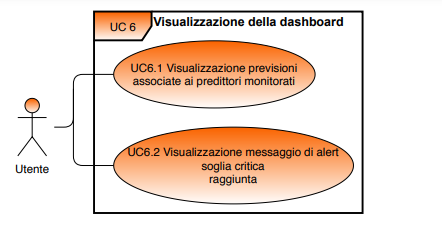
\includegraphics[scale=0.80]{../Analisi_dei_requisiti/img/Diagrammi_UML/UC9_Visualizzazione_della_dashboard.png}
	%	\caption{Visualizzazione delle previsioni}
	%\end{figure}

		\begin{itemize}
			\item\textbf{Codice Identificativo}: UC10;
			\item\textbf{Titolo}: Visualizzazione della dashboard;
			\item\textbf{Attore primario}: utente generico;
			\item\textbf{Descrizione}: attività in cui viene visualizzata la dashboard contenente il pannello relativo al plugin \textit{Predire in Grafana}. Il pannello visualizza le previsioni per ogni collegamento, calcolate sui dati forniti in input dal datasource precedentemente configurato dall'utente. Ogni collegamento è marcato con una colorazione differente per individuare più facilmente la serie temporale della previsione relativa a ciascun collegamento. La dashboard viene aggiornata continuamente in base ai dati in ingresso. \'E possibile, tramite le impostazioni di Grafana, impostare il tempo dopo il quale viene riaggiornata la dashboard (di default settato a "Off" e quindi manuale) e il tempo entro il quale vengono visualizzate le previsioni (di default settato alle ultime 6 ore); 
			\item\textbf{Precondizioni}: 
			\begin{enumerate}
				\item l'utente visualizza la dashboard a cui è stato aggiunto il plugin \textit{Predire in Grafana};
				\item l'utente ha avviato correttamente il monitoraggio del flusso dati (\hyperref[par:UC7.2]{UC7.2}) con relativi predittori collegati.
			\end{enumerate}				
			\item\textbf{Postcondizioni}: il sistema mantiene aggiornate e visualizzabili, attraverso l'uso delle dashboard, le misurazioni e le previsioni dei predittori associati da parte dell'utente;
			\item\textbf{Scenario principale}: 
			\begin{enumerate}
				\item (\hyperref[par:UC10.1]{UC10.1}) l'utente visualizza le previsioni calcolate nella dashboard di Grafana;
				\item (\hyperref[par:UC10.2]{UC10.2}) ogni volta che una soglia critica viene attivata dai dati di previsioni viene visualizzato un messaggio di alert.
			\end{enumerate}
				
		\end{itemize}
		
		\label{par:UC10.1}
	\subsubsection{UC10.1 - Visualizzazione previsioni}
		\begin{itemize}
			\item\textbf{Codice Identificativo}: UC10.1;
			\item\textbf{Titolo}: Visualizzazione previsioni;
			\item\textbf{Attore primario}: utente generico;
			\item\textbf{Descrizione}: attività in cui vengono visualizzate nella dashboard le previsioni sul flusso dati per ogni collegamento impostato in precedenza dall'utente;
			\item\textbf{Precondizioni}: l'utente ha avviato correttamente il monitoraggio del flusso dati (\hyperref[par:UC7]{UC7}) con relativi predittori collegati;
			\item\textbf{Postcondizioni}: l'utente ha visualizzato sulla dashboard le previsioni calcolate precedentemente;
			\item\textbf{Scenario principale}: l'utente visualizza le previsioni calcolate. Il sistema si aggiorna costantemente grazie ai dati provenienti dal database, effettuando l'operazione di calcolo delle previsioni sul flusso dati associato ai predittori. Tale operazione di calcolo di previsione viene eseguito in base alla politica temporale stabilita impostata sulla piattaforma Grafana;
		\end{itemize}
			
		
		\label{par:UC10.2}
	\subsubsection{UC10.2 - Visualizzazione messaggio di alert "Soglia critica raggiunta"}
		\begin{itemize}
			\item\textbf{Codice Identificativo}: UC10.2;
			\item\textbf{Titolo}: Visualizzazione messaggio di alert "Soglia critica raggiunta";
			\item\textbf{Attore primario}: utente generico;
			\item\textbf{Descrizione}: attività in cui viene visualizzato un alert di soglia critica raggiunta ogniqualvolta che una soglia impostata su un collegamento venga superata;
			\item\textbf{Precondizioni}: una delle soglie impostate per il predittore (\hyperref[par:UC3.4]{UC3.4}) è stata raggiunta o superata;
			\item\textbf{Postcondizioni}: l'utente ha visualizzato il messaggio di alert riguardante la soglia interessata;
			\item\textbf{Scenario principale}:
				\begin{enumerate}
					\item l'utente visualizza il messaggio di alert "Soglia critica raggiunta" in cui viene segnalato che una soglia impostata nel processo di collegamento dei predittori al flusso dati (\hyperref[par:UC3.4]{UC3.4}) è stata raggiunta o superata;
					\item l'utente clicca il pulsante "X" per proseguire.		
				\end{enumerate}		
		\end{itemize}
	
% - Casi d'uso: Estensioni - %%%%%%%%%%%%%%%%%%%%%%%%%%%%%%%%%%%
	\label{par:UC11}
	\subsection{UC11 - Visualizzazione messaggio d'errore "Nessun file CSV caricato"}
		\begin{itemize}
			\item\textbf{Codice Identificativo}: UC11;
			\item\textbf{Titolo}: Visualizzazione messaggio d'errore "Nessun file CSV caricato";
			\item\textbf{Attore primario}: utente generico;
			\item\textbf{Precondizioni}: l'utente ha cliccato il pulsante di conferma (\hyperref[par:UC1.4]{UC1.4}) senza aver caricato un file CSV contenente i valori utilizzati per l'addestramento (\hyperref[par:UC1.1]{UC1.1});
			\item\textbf{Postcondizioni}: l'utente visualizza l'errore, viene quindi riportato alla finestra di selezione del file CSV (\hyperref[par:UC1.1]{UC1.1});
			\item\textbf{Scenario principale}: l'utente visualizza il messaggio d'errore "Nessun file CSV caricato" in cui viene segnalato il fatto che non è stato caricato alcun file CSV (\hyperref[par:UC1.1]{UC1.1}) e quindi non si può procedere con l'addestramento; 		
		\end{itemize}
		
%%%%%%%%%%%%%%%%%%%%%%%%%%%%%%%%%%%%%%%%%%%
		
	\label{par:UC12}
	\subsection{UC12 - Visualizzazione messaggio d'errore "Nessun algoritmo selezionato"}
		\begin{itemize}
			\item\textbf{Codice Identificativo}: UC12;
			\item\textbf{Titolo}: Visualizzazione messaggio d'errore "Nessun algoritmo selezionato";
			\item\textbf{Attore primario}: utente generico;
			\item\textbf{Precondizioni}: l'utente ha cliccato il pulsante di conferma (\hyperref[par:UC1.4]{UC1.4}) senza aver scelto un algoritmo dalla Combo Box (\hyperref[par:UC1.2]{UC1.2});
			\item\textbf{Postcondizioni}: l'utente visualizza l'errore, viene quindi riportato alla scelta dell'algoritmo (\hyperref[par:UC1.2]{UC1.2});
			\item\textbf{Scenario principale}: l'utente visualizza il messaggio d'errore "Nessun algoritmo selezionato" in cui viene segnalato il fatto che non è stato scelto alcun algoritmo da addestrare (\hyperref[par:UC1.2]{UC1.2}) e quindi non si può procedere con l'addestramento; 		
		\end{itemize}
		
%%%%%%%%%%%%%%%%%%%%%%%%%%%%%%%%%%%%%%%%%%%%%%
		
	\label{par:UC13}
	\subsection{UC13 - Visualizzazione messaggio d'errore "File CSV incompatibile"}
		\begin{itemize}
			\item\textbf{Codice Identificativo}: UC13;
			\item\textbf{Titolo}: Visualizzazione messaggio d'errore "File CSV incompatibile";
			\item\textbf{Attore primario}: utente generico;
			\item\textbf{Precondizioni}: l'utente ha selezionato il file CSV che intende utilizzare per l'addestramento e ha cliccato il pulsante di conferma. Il file selezionato è strutturalmente errato e non c'è compatibilità con l'algoritmo selezionato;
			\item\textbf{Postcondizioni}: l'utente visualizza l'errore, viene quindi riportato alla finestra di selezione del file CSV (\hyperref[par:UC1.1]{UC1.1});
			\item\textbf{Scenario principale}: l'utente visualizza il messaggio d'errore "File incompatibile" in cui viene segnalato il fatto che il file CSV da lui selezionato (\hyperref[par:UC1.1]{UC1.1}) non è adatto per l'addestramento; 		
		\end{itemize}

%%%%%%%%%%%%%%%%%%%%%%%%%%%%%%%%%%%%%%%%%%%%


\label{par:UC14}
	\subsection{UC14 - Visualizzazione messaggio d'errore "Collega tutti i predittori"}
		\begin{itemize}
			\item\textbf{Codice Identificativo}: UC14;
			\item\textbf{Titolo}: Visualizzazione messaggio d'errore "Collega tutti i predittori";
			\item\textbf{Attore primario}: utente generico;
			\item\textbf{Descrizione}: attività in cui viene visualizzato un messaggio d'errore che segnala all'utente di collegare tutti i predittori per poter inserire correttamente un nuovo collegamento;
			\item\textbf{Precondizioni}: l'utente ha confermato le selezioni per il collegamento di un predittore ad un nodo del flusso (\hyperref[par:UC3.5]{UC3.5}) e non ha collegato tutti i predittori ad un nodo del flusso dati;
			\item\textbf{Postcondizioni}: 
				\begin{enumerate}
					\item l'utente visualizza il messaggio di errore dove viene segnalato di collegare tutti i predittori;
					\item le scelte dell'utente precedenti non vengono finalizzate e non viene creato il collegamento.
				\end{enumerate}		
			\item\textbf{Scenario principale}:
				\begin{enumerate}
					\item l'utente visualizza il messaggio d'errore "Collega tutti i predittori" in cui viene segnalato che è necessario collegare tutti i predittori ad un nodo del flusso dati per creare un collegamento(\hyperref[par:UC3]{UC3});
					\item l'utente clicca il pulsante "X" per proseguire.		
				\end{enumerate}		
		\end{itemize}

%%%%%%%%%%%%%%%%%%%%%%%%%%%%%%%%

%NON IMPLEMENTATO
		\label{par:UC15}
	\subsection{UC15 - Visualizzazione messaggio d'errore "Soglia non valida"}
		\begin{itemize}
			\item\textbf{Codice Identificativo}: UC15;
			\item\textbf{Titolo}: Visualizzazione messaggio d'errore "Soglia non valida";
			\item\textbf{Attore primario}: utente generico;
			\item\textbf{Precondizioni}: l'utente ha impostato una soglia di monitoraggio(\hyperref[par:UC3.4]{UC3.4}) non valida per contenuto o formato;
			\item\textbf{Postcondizioni}: l'utente visualizza il messaggio d'errore sulla soglia appena impostata;		
			\item\textbf{Scenario principale}:
				\begin{enumerate}
					\item l'utente visualizza il messaggio d'errore "Soglia non valida" in cui viene segnalato che la soglia appena inserita (\hyperref[par:UC3.4]{UC3.4}) non può essere accettata e viene invitato ad inserirla nuovamente;
					\item l'utente clicca il pulsante "Conferma" per proseguire e viene riportato all'inserimento della soglia.		
				\end{enumerate}		
		\end{itemize}

%%%%%%%%%%%%%%%%%%%%%%%%%%%%%%%
	\label{par:UC16}
	\subsection{UC16 - Visualizzazione messaggio d'errore "Inserisci un nome per la connessione"}
		\begin{itemize}
			\item\textbf{Codice Identificativo}: UC16;
			\item\textbf{Titolo}: Visualizzazione messaggio d'errore "Inserisci un nome per la connessione";
			\item\textbf{Attore primario}: utente generico;
			\item\textbf{Descrizione}: attività in cui viene visualizzato un messaggio d'errore che segnala all'utente di inserire un nome identificativo al collegamento per poterlo inserire correttamente nella lista dei collegamenti;
			\item\textbf{Precondizioni}: l'utente ha confermato le selezioni per il collegamento di un predittore ad un nodo del flusso (\hyperref[par:UC3.5]{UC3.5}) ed non ha inserito un nome identificativo per il collegamento;
			\item\textbf{Postcondizioni}:
				\begin{enumerate}
					\item l'utente visualizza il messaggio di errore dove viene segnalato di assegnare un nome per il collegamento;
					\item le scelte dell'utente precedenti non vengono finalizzate e non viene creato il collegamento.
				\end{enumerate}		
			\item\textbf{Scenario principale}:
				\begin{enumerate}
					\item l'utente visualizza il messaggio d'errore "Inserisci un nome per la connessione" in cui viene segnalato che che è necessario collegare inserire un nome identificativo per creare un collegamento (\hyperref[par:UC3]{UC3});
					\item l'utente clicca il pulsante "X" per proseguire.		
				\end{enumerate}		
		\end{itemize}

%%%%%%%%%%%%%%%%%%%%%%%%%%%%%%%%%%%%%%

\label{par:UC17}
	\subsection{UC17 - Visualizzazione messaggio d'errore "Attenzione monitoraggio attivo!"}
		\begin{itemize}
			\item\textbf{Codice Identificativo}: UC17;
			\item\textbf{Titolo}: Visualizzazione messaggio d'errore "Attenzione monitoraggio attivo!";
			\item\textbf{Attore primario}: utente generico;
			\item\textbf{Descrizione}: attività in cui viene visualizzato un messaggio d'errore che segnala all'utente l'impossibilità di eliminare o modificare un collegamento perché il monitoraggio delle previsioni è attualmente attivo;
			\item\textbf{Precondizioni}: l'utente ha cliccato il pulsante di eliminazione (\hyperref[par:UC5.1]{UC5.1}) o il pulsante di modifica (\hyperref[par:UC6.1]{UC6.1}) di un collegamento quando il monitoraggio è attivo;
			\item\textbf{Postcondizioni}: 
				\begin{enumerate}
					\item l'utente ha visualizzato il messaggio di errore dove viene segnalata l'impossibilità di eliminare o modificare un collegamento perché il monitoraggio delle previsioni è attualmente attivo;
					\item l'utente viene riportato alla visualizzazione della lista dei collegamenti disponibili (\hyperref[par:UC4]{UC4}).
				\end{enumerate}		
			\item\textbf{Scenario principale}:
				\begin{enumerate}
					\item l'utente visualizza il messaggio d'errore "Attenzione monitoraggio attivo!" in cui viene segnalato che non è possibile modificare (\hyperref[par:UC6]{UC6}) o eliminare (\hyperref[par:UC5]{UC5}) il collegamento selezionato perché il monitoraggio è attivo;
					\item l'utente clicca il pulsante "X" per proseguire.		
				\end{enumerate}		
		\end{itemize}

%%%%%%%%%%%%%%%%%%%%%%%%%%%%%%%%%%%%%%

		\label{par:UC18}
	\subsection{UC18 - Visualizzazione messaggio d'errore "Nessun predittore collegato"}
		\begin{itemize}
			\item\textbf{Codice Identificativo}: UC18;
			\item\textbf{Titolo}: Visualizzazione messaggio d'errore "Nessun predittore collegato";
			\item\textbf{Attore primario}: utente generico;
			\item\textbf{Precondizioni}: l'utente ha avviato il monitoraggio (\hyperref[par:UC7]{UC7}), senza aver impostato alcun collegamento (\hyperref[par:UC3]{UC3});
			\item\textbf{Postcondizioni}:
				\begin{enumerate}
					\item l'utente ha visualizzato il messaggio d'errore sulla mancata presenza di collegamenti;	
					\item	il monitoraggio non viene avviato.
				\end{enumerate}
			\item\textbf{Scenario principale}:
				\begin{enumerate}
					\item l'utente visualizza il messaggio d'errore "Nessun predittore collegato" in cui viene segnalato che non è stata inserito alcun collegamento tra predittore e flusso dati;
					\item l'utente clicca il pulsante "X" per proseguire e viene riportato all'impostazione di collegamento predittori (\hyperref[par:UC3]{UC3}).		
				\end{enumerate}		
		\end{itemize}


	
%%%%%%%%%%%%%%%%%%%%%%%%%%%%%%%








